\documentclass[usenames,dvipsnames]{beamer}


\usepackage{soul}

\usepackage{tikz}
\usepackage{pgfplots}

\usepackage{subfigure}




\usepackage{xspace}
\usepackage{graphicx}
\usepackage{epsfig}
\usepackage{verbatim}


%\usepackage{algorithm}
%\usepackage[noend]{algpseudocode}
\newcommand{\todo}[1]{{\color{red}\textbf{\hl{#1}}\xspace}}


\usepackage[ruled,vlined]{algorithm2e}

\usepackage{float}

%\usetheme{Columbus}
\usetheme{Madrid}
 \setbeamertemplate{navigation symbols}{}
 \setbeamercovered{transparent}

\newcommand{\card}[1]{\ensuremath{|#1|}}
\newcommand{\union}{\ensuremath{\cup}}

\newcommand{\ceil}[1]{\left\lceil#1\right\rceil}
\newcommand{\floor}[1]{\lfloor#1\rfloor}

\usealerttemplate{\color{red}\bf}{}

\graphicspath{{fig/}}

\title[Uncertain Scheduling]{Replicated Data Placement for Uncertain Scheduling}

\date[APDCM 2015]{APDCM 2015\\May 25th}

\author[Erik Saule]{ Manmohan Chaubey$^1$,{\bf Erik Saule}$^1$}
 
\institute[UNCC]{ mchaubey@uncc.edu, esaule@uncc.edu\\
  $^1$ University of North Carolina at Charlotte, Computer Science
}


\begin{document}

\maketitle

\begin{frame}
  \frametitle{Outline}
  \tableofcontents[subsectionstyle=hide/hide/hide]
\end{frame}

\section{Introduction}

\AtBeginSection[]
{
  \begin{frame}<beamer>
    \frametitle{Outline}
    \tableofcontents[currentsection,subsectionstyle=hide/hide/hide]
  \end{frame}
}

\subsection{Motivation}

\begin{frame}
  \frametitle{Uncertainty in Scheduling}

  \begin{itemize}
  \item Scheduling is a common tool to manage load balance
  \item Often make many assumptions
    \begin{itemize}
    \item Release date are known (offline/online), or release ``rates''
    \item All machines are the same (or predictabily heterogeneous)
    \item Processing times are known
    \end{itemize}
  \item All of these assumptions are typically incorrect
    \begin{itemize}
    \item Release dates are unknown, release rates are not ``constant''
    \item Machines slightly differ
    \item Processing times are either unknown or estimated
    \end{itemize}
  \end{itemize}

  \pause

  \begin{center}
    {\Large How can scheduling account for this?}

    Ready to simplify the problem for the investigation
  \end{center}
  
\end{frame}

\begin{frame}
  \frametitle{Data Placement}
  
  \begin{itemize}
  \item If there was cost-free migration, many techniques apply:
    \begin{itemize}
    \item Having a shared work queue
    \item Workstealing
    \end{itemize}
  \item Data locality makes the difference
    \begin{itemize}
      \item If you do not have the data, you can not compute
      \item You need to access them somehow
    \end{itemize}
  \item In many applications tasks are ``pinned'' to a particular machine
    \begin{itemize}
    \item with dynamic data (i.e. Particle in Cell) little can be done
    \item opportunities with static data (Hadoop, DOoC+LAF, Out of Core)
    \end{itemize}
  \end{itemize}

  \pause
  
  \begin{block}{This paper}
    \begin{itemize}
    \item Where to place the (mostly static) data to manage uncertainty?
    \item Can replicating the data of some tasks help ?
    \end{itemize}
  \end{block}
\end{frame}

\section{Model}

\subsection{Notations}

\begin{frame}
  \frametitle{Notations}

  \begin{block}{Model}
    \begin{itemize}
    \item $m$ machines
    \item $n$ tasks
    \item Estimated processing time $\tilde{p}_j$
    \item Imprecision factor $\alpha \geq 1$
    \item Real (unknown) processing time $p_j$ are such that $\frac{\tilde{p}_{j}}{\alpha}\leq p_{j}\leq \alpha \tilde{p}_{j}$
    \end{itemize}
  \end{block}
  
  \pause

  \begin{block}{Is $\alpha$ reasonable?}
    Depends on where the uncertainty comes from
    \begin{itemize}
    \item Variability in processing power (cloud allocation)
    \item Models often predicts range of performance (SpMV out of nnz)
    \item Guesses in predicted performance
    \item System jitter
    \end{itemize}
  \end{block}
  
\end{frame}

\subsection{2 Phases Algorithms}

\begin{frame}
  \frametitle{A Two Sided Problem}

  \begin{block}{Scheduling model}
    \begin{itemize}
    \item Phase 1: Offline data placement
      \begin{itemize}
      \item The algorithm decides where each task data will be
        replicated
      \item Purely offline and only uses processing time estimates $\tilde{p}_j$
      \end{itemize}
    \item Phase 2: Online semi clairvoyant scheduling
      \begin{itemize}
      \item A task can only be scheduled where its data is available
      \item Scheduling happens based on estimate $\tilde{p}_j$
      \item The actual processing time $p_j$ is only known when the task completes
      \end{itemize}
    \end{itemize}

    Applications: all large data iterative problems
  \end{block}
  
  \begin{block}{Goals}
    \begin{itemize}
    \item Minimize replication
    \item Minimize makespan
    \end{itemize}
  \end{block}
\end{frame}


\section{Strategy 1: No Replication}

\subsection{Lower Bound}

\begin{frame}
  \frametitle{No better than $\frac{\alpha^{2}m }{\alpha^{2} + m-1} \approx \alpha^2$}

  \begin{itemize}
  \item The adversary sends tasks of identical size
  \item The adversary identifies the most loaded processor in the solution
  \item The tasks on the most loaded processor are increased by $\alpha$
  \item Others are shrunk by $\alpha$
  \item The best algorithm will balance the tasks
  \end{itemize}
  
  \begin{center}
    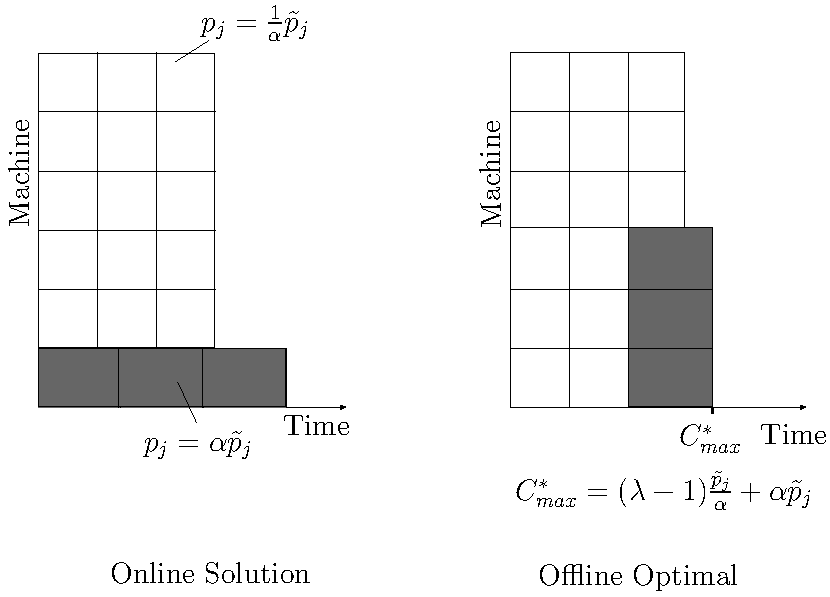
\includegraphics[width=.6\linewidth]{figs/model1.pdf}
  \end{center}
\end{frame}

\subsection{LPT-No choice}

\begin{frame}
  \frametitle{LPT-No choice}

  \begin{block}{Algorithm}
    Phase 1: (Distribute the data to a single machine)
    \begin{itemize}
    \item Use Largest Processing Time on estimated processing times $\tilde{p}_j$
    \end{itemize}
    Phase 2:
    \begin{itemize}
    \item Schedule tasks in any order where they are pinned
    \end{itemize}
  \end{block}

  \pause

  \begin{block}{LPT-No choice is $\frac{2\alpha^{2}m}{2\alpha^{2}+ m-1}$-competitive}
    \begin{itemize}
    \item List Scheduling on estimated processing time:
      $\tilde C_{max}\leq  \frac{\sum{\tilde p_j + (m-1) \tilde p_l} }{m}$
    \item Increase critical tasks: $C_{max}\leq \alpha \tilde C_{max}\leq \alpha \left ( \frac{\sum{\tilde p_j + (m-1) \tilde p_l} }{m} \right )$
    \item Shrink non critical tasks: $ \sum {p_j} = \frac{\sum \tilde{p_j}- \tilde{C_{max}}}{\alpha} + \alpha \tilde C_{max}$
    \item Perfect balance condition: $m C_{max}^{*}\geq \frac{m-1}{\alpha m} \left( \sum \tilde p_j - \tilde{p_l} \right) + {C_{max}}$

    \item LPT guarantees $\sum \tilde p_j-\tilde p_l \geq m (\tilde C_{max}-\tilde p_l)$ and $\tilde{p_l} \leq \frac{\tilde{C}_{max}}{2}$
    \end{itemize}
    
  \end{block}
\end{frame}

\section{Strategy 2: Replicate Everywhere}

\subsection{LPT-No Restriction}

\begin{frame}
  \frametitle{LPT-No Restriction}

  \begin{block}{Algorithm}
    Phase 1:
    \begin{itemize}
    \item Replicate all tasks on all machines
    \end{itemize}
    Phase 2:
    \begin{itemize}
    \item Sort tasks in non-increasing estimated processing time $\tilde{p}_j$
    \item Schedule tasks online as soon as possible
    \end{itemize}
  \end{block}
  
  \pause

  \begin{block}{LPT-No Restriction is $\min(2-\frac{1}{m}, 1 + (\frac{m-1}{m}) \frac{\alpha^{2}}{2})$-competitive}
    \begin{itemize}
    \item By property of List Scheduling : $C_{max} \leq  \frac{\sum {p_j}}{m} + \frac{(m-1)}{m}p_l$
    \item Lower bound: $C_{max}^{*}\geq\frac{\sum p_j}{m}$
    \item Ratio: $\frac{C_{max}}{C_{max}^{*}} \leq 1 + {\frac{m-1}{m}}\left(\frac{p_l}{C_{max}^{*}}\right)$
    \item If there are two tasks on the most loaded machine then $C_{max}^* \geq {\frac{2}{\alpha^{2}}} p_l$
    \end{itemize}
  \end{block}  
\end{frame}

\section{Strategy 3: Replicate in Groups}

\subsection{LS-Groups}

\begin{frame}
  \frametitle{LS groups}

  \begin{block}{Algorithm}
    Phase 1:
    \begin{itemize}
    \item Partition the machines in $k$ groups
    \item Allocate the task to the groups with List Scheduling
    \item Replicate the data of each task on all the groups it is allocated to
    \end{itemize}
    
    Phase 2:
    \begin{itemize}
    \item Use List Scheduling in each group
    \end{itemize}    
  \end{block}
  
  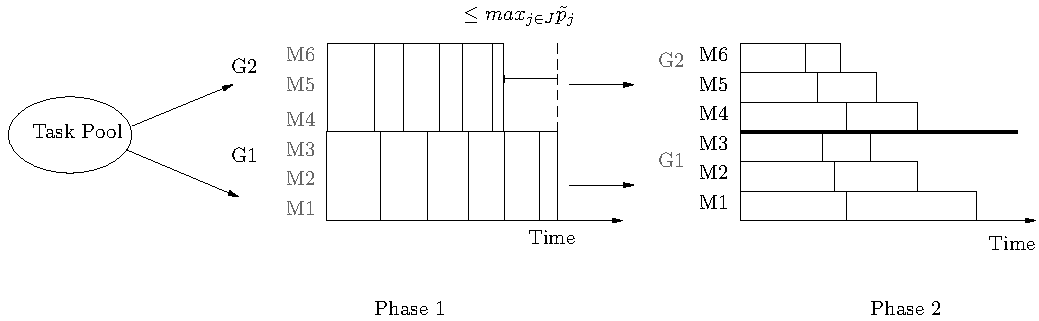
\includegraphics[width=\textwidth]{figs/model3.pdf}
\end{frame}

\begin{frame}
  \frametitle{LS groups is $ \frac{k\alpha^{2}}{\alpha^{2}+k-1} (1+
    \frac{k-1}{m} ) + \frac{m-k}{m}$-competitive }
  
  
  \begin{itemize}
  \item Without loss of generality, Group 1 is most loaded
  \item Lower bound can be written as:
    $C_{max}^{*} \geq  \frac{\sum_{j \in G1 }^{}{{p_{j}}}+ \sum_{l=2}^{k}\sum_{j \in Gl }^{}{{p_{j}}}}{m}$
  \item List scheduling in phase 2: $C_{max} \leq \frac{\sum_{j \in G1 }^{}{{p_{j}}}}{m/k} + {\frac{m/k-1}{m/k}} p_{max}$
  \item Almost balanced at the end of phase 1: $\left | (k-1)\sum_{j \in G1 }^{}{\tilde p_{j}}- \sum_{l=2}^{k}\sum_{j \in Gl }^{}{\tilde p_{j}} \right | \leq (k-1) {max_{j \in J}}{\tilde p_{j}}$
  \pause
  \item Case 1: $(k-1)\sum_{j \in G1 }^{}{\tilde p_{j}} >
  \sum_{l=2}^{k}\sum_{j \in Gl }^{}{\tilde p_{j}}$
    \begin{itemize}
      \item Quality of the estimation: $\sum_{l=2}^{k}\sum_{j \in Gl }^{}{{p_{j}}} \geq (k-1) \left(\frac{1}{\alpha^{2}}\sum_{j \in G1 }^{}{{p_{j}}}-  {max_{j \in J}}{{p_{j}}} \right)$
      \item Mashing all together
    \end{itemize}
    \pause
  \item Case 2: $(k-1)\sum_{j \in G1 }^{}{\tilde p_{j}} \leq \sum_{l=2}^{k}\sum_{j \in Gl }^{}{\tilde p_{j}}$
    \begin{itemize}
    \item Quality of the estimation : $\sum_{l=2}^{k}\sum_{j \in Gl }^{}{ p_{j}} \geq \frac{1}{\alpha^2} (k-1)\sum_{j \in G1 }^{}{ p_{j}}$
    \item Mashing all together
    \end{itemize}

  \end{itemize}
\end{frame}



\section{Conclusion}

\subsection{Summary}

\begin{frame}
  \frametitle{All results}
  
  \begin{center}

    \begin{tabular}{|l|c|c|c|c|c|}
      \hline
      Replication & Approximation ratio  \\
      \hline
      $|M_j|=1$ & $\frac{C_{max}}{C_{max}^{*}}\leq \frac{2\alpha^{2}m}{2\alpha^{2}+ m-1}$ \\
      & No approximation better than $\frac{\alpha^{2}m }{\alpha^{2} + m-1}$  \\
      
      \hline
      $|M_j|=m$ & $\frac{C_{max}}{C_{max}^{*}} \leq 1 + (\frac{m-1}{m})\frac{\alpha^{2}}{2}$  \\
      & $\frac{C_{max}}{C_{max}^{*}} \leq 2-\frac{1}{m}$ [Graham66]   \\
      \hline
      
      $|M_j|= \frac{m}{k} $ & $\frac{C_{max}}{C_{max}^{*}} \leq \frac{k\alpha^{2}}{\alpha^{2}+k-1} \left(1+ {\frac{k-1}{m}} \right)+ {\frac{m-k}{m}}$ \\
      
      \hline
    \end{tabular}
  \end{center}
\end{frame}

\begin{frame}
  \frametitle{All results - With numbers}

  \vspace{-1.5em}

  \begin{columns}
    \column{.49\linewidth}

    \begin{center}
      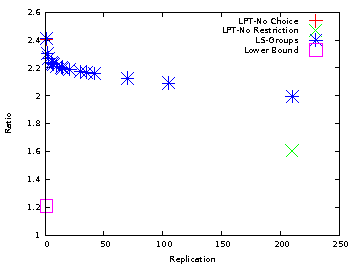
\includegraphics[width=\textwidth]{figs/alpha_11.pdf}
      
      {\footnotesize $m=210$, $\alpha=1.1$}
    \end{center}
    
    \column{.49\linewidth}

    % \column{.4\linewidth}
  
    % \begin{center}
    %   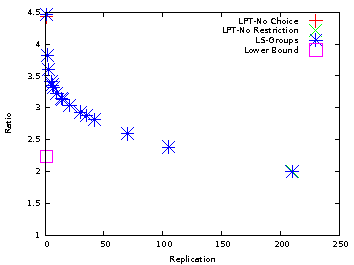
\includegraphics[width=\textwidth]{figs/alpha_15.pdf}

    %   {\footnotesize $m=210$, $\alpha=1.5$}
    % \end{center}

    \begin{center}
      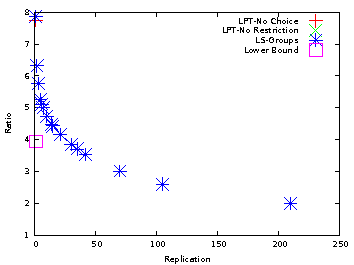
\includegraphics[width=\textwidth]{figs/alpha_2.pdf}
  
      {\footnotesize $m=210$, $\alpha=2$}
    \end{center}


    
  \end{columns}

%  \vspace{-1.1em}

    \begin{block}{Remarkables}
      \begin{itemize}
      \item Tradeoffs are found by LS-Groups
      \item LS-Groups might benefit from LPT for low $\alpha$
      \item Few replication can make a large difference
      \item Replication allows to guarantee better than no replication lower bound
      \end{itemize}
    \end{block}
  
\end{frame}

\subsection{Conclusion and Future Works}

\begin{frame}
  \frametitle{Conclusion and Future Works}

  \begin{block}{Conclusion (aka What does it all mean?)}
    \begin{itemize}
    \item Identified a new lower bound for the problem and provided guaranteed algorithms
    \item The algorithm can leverage the tradeoff between replication and load balance guarantee
    \item Imbalance caused by uncertainty can be fought by enabling tasks to execute on more machines
    \item Even few replications can alleviate the problem cause by uncertainty on load balance 
    \end{itemize}
  \end{block}

  \pause

  \begin{block}{Future works}
    \begin{itemize}
    \item Can more complex strategy help?
    \item Better lower bounds? (In particular for replicate everywhere)
    \item Some replication are more ``expensive''
    \item In brief, look at more realistic models
    \end{itemize}
  \end{block}
\end{frame}



\begin{frame}
  \frametitle{Thank you}

    \begin{block}{More information}
    contact : esaule@uncc.edu
    
    visit: \url{http://webpages.uncc.edu/~esaule}
  \end{block}

\end{frame}


\end{document}
